\notechapter{N-20221207}{Set Problems, Extremal Counting, and Venn-Diagram Reasoning}

\section{A set construction problem}

The first problem defines a finite set
\[
  A=\{a_1<a_2<\cdots<a_k\}
\]
of positive integers and builds two derived sets, one from sums and one from differences.  The handwritten solution records the important idea: use the union \(S\cup T\), and do not try to identify every element exactly.  Bound its size from below and above.

The sum set contains at least the ordered chain
\[
  2a_1,\ a_1+a_2,\ 2a_2,\ldots,\ a_{k-1}+a_k,\ 2a_k,
\]
so
\[
  |S|\ge2k-1.
\]
The difference set contains
\[
  0,\ a_2-a_1,\ a_3-a_1,\ldots,\ a_k-a_1,
\]
so
\[
  |T|\ge k.
\]
Under the condition of the problem, \(S\cap T=\varnothing\), hence
\[
  |S\cup T|=|S|+|T|\ge3k-1.
\]
On the other hand, all these numbers lie between \(0\) and \(2a_k\), so
\[
  |S\cup T|\le2a_k+1.
\]
Thus
\[
  3k-1\le2a_k+1.
\]
If \(a_k\le2021\), then
\[
  k\le\frac{2\cdot2021+2}{3}=1348.
\]
The construction
\[
  A=\{674,675,\ldots,2021\}
\]
attains this bound, so the maximum is
\[
  |A|=1348.
\]

\section{What this problem teaches}

The note's blue comment says that using \(S\cup T\) is a good way to avoid proving a complicated extremal statement directly.  This is the key lesson.  When a problem asks for the largest possible size of a set, it often helps to build auxiliary sets whose sizes are forced by the structure.

A lower bound comes from a construction.  An upper bound comes from counting constraints.  A complete solution needs both.

\section{A Venn-diagram necessary-and-sufficient problem}

Another problem defines set difference
\[
  A-B=\{x:x\in A,\ x\notin B\}
\]
and asks for the relation among \(A,B,C\) when
\[
  (A-B)\cup(B-A)\subseteq C.
\]
The question asks whether this is equivalent to a condition involving
\[
  A\subseteq(C-B)\cup(B-C)
\]
or
\[
  A\cap B\cap C=\varnothing.
\]

The handwritten solution first draws a Venn diagram, then rewrites the pieces algebraically.  The symmetric difference
\[
  (A-B)\cup(B-A)
\]
is the part where membership in \(A\) and \(B\) differs.  If this is contained in \(C\), then outside \(C\) the sets \(A\) and \(B\) must agree.

The correct way to solve such problems is to analyze each of the eight Venn regions.  The note records a false start and then corrects it, which is valuable: set identities are easy to get wrong if one reasons only verbally.

\begin{figure}[H]
\centering
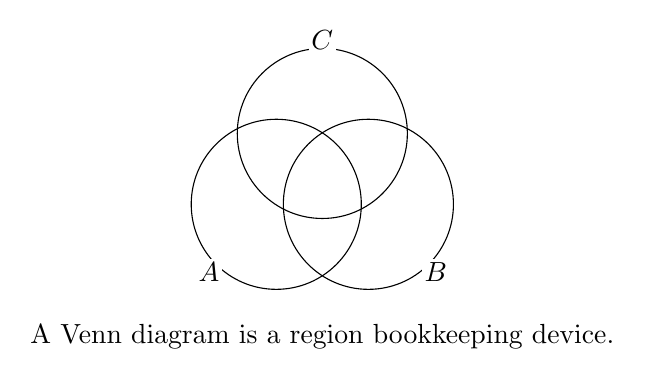
\begin{tikzpicture}[scale=0.9,every node/.style={fill=white,inner sep=1pt}]
  \draw (0,0) circle (1.2);
  \draw (1.3,0) circle (1.2);
  \draw (0.65,1.0) circle (1.2);
  \node at (-0.95,-0.95) {$A$};
  \node at (2.25,-0.95) {$B$};
  \node at (0.65,2.32) {$C$};
  \node[below] at (0.65,-1.65) {A Venn diagram is a region bookkeeping device.};
\end{tikzpicture}
\caption{For three sets one should reason region by region, not by visual guesswork alone.}
\end{figure}

\section{Difference identities}

One useful identity appearing in the handwritten reasoning is
\[
  B-C=B\cap C^c.
\]
Therefore
\[
  B-C-(A\cap B)
  =
  B\cap C^c\cap(A\cap B)^c.
\]
Using De Morgan,
\[
  (A\cap B)^c=A^c\cup B^c,
\]
so
\[
  B\cap C^c\cap(A^c\cup B^c)
  =
  (B\cap C^c\cap A^c)\cup(B\cap C^c\cap B^c).
\]
The second term is empty, hence
\[
  B-C-(A\cap B)=B\cap A^c\cap C^c.
\]
This is exactly the kind of algebraic cleanup that a Venn diagram suggests but does not replace.

\section{Coordinate and algebraic exercises}

The later pages contain a mixture of algebraic and coordinate exercises.  They include problems about quadratic expressions, tangent or chord diagrams, and conditions that must be translated into equations.  The handwritten computations repeatedly use the same pattern:
\begin{enumerate}[(i)]
  \item introduce the unknowns explicitly;
  \item translate each condition into an equation or inequality;
  \item reduce by substitution or by completing the square;
  \item check equality or boundary cases.

\end{enumerate}

Several sketches show lines touching curves or intersecting regions.  Rather than reproducing them as raw images, the important content is the method: a picture tells us which algebraic condition to impose, such as tangency, parallelism, or containment.

\section{A note on proof writing}

The red handwritten reflection says that a purely diagrammatic method is intuitive but can be unreliable.  The mature solution uses the diagram to discover the statement, then uses set algebra to prove it.  This is an excellent general lesson.  Geometry and diagrams are for finding the path; formal manipulations are for making the path safe.


\section{Extremal set problems: why constructions matter}

In an extremal counting problem, an upper bound is only half the solution.  One must also give a construction showing the bound is sharp.  The note's sum-set and difference-set arguments follow this pattern: first prove that the derived sets must contain enough elements; then exhibit a set \(A\) for which the lower bound is actually attained.

This is a common combinatorial habit.  Inequalities show impossibility beyond a threshold.  Constructions show that the threshold is real.

\section{Venn diagrams versus proofs}

Venn diagrams are excellent for discovering set identities, but the proof should eventually be written elementwise.  For example,
\[
  A\setminus(B\cup C)=(A\setminus B)\cap(A\setminus C)
\]
is proved by taking an arbitrary \(x\) and translating membership:
\[
  x\in A\setminus(B\cup C)
  \Longleftrightarrow
  x\in A,\ x\notin B,\ x\notin C.
\]
This is exactly the condition for membership in the right-hand side.  The diagram gives intuition; the element chase gives proof.

\section{Expanded synthesis and advanced context}

This note is about extremal and logical reasoning.  The extremal problem uses auxiliary sets and cardinality bounds.  The Venn problem uses Boolean algebra and region decomposition.  Both are early forms of a common method: replace a vague configuration by a finite list of regions or quantities that can be counted exactly.  This is the same spirit behind combinatorial proofs, measure decompositions, and even sigma-algebra calculations later in analysis.



\paragraph{Expanded synthesis.}
The elementary geometric content of this chapter should be read through transformations and invariants. The earlier sections (`A set construction problem`, `What this problem teaches`, `A Venn-diagram necessary-and-sufficient problem`, `Difference identities`, `Coordinate and algebraic exercises`) may use coordinates, angles, determinants, parametrizations, or integral formulas, but the organizing question is: which quantities survive the transformations naturally associated with the problem? Euclidean geometry preserves distances and angles; affine geometry preserves lines and ratios on a line; projective geometry preserves incidence and cross ratio; differential geometry preserves coordinate-independent objects such as forms, metrics, and orientations.

This perspective separates different layers of a problem. A dot product belongs to metric geometry. A determinant belongs to oriented volume. A cross ratio belongs to projective geometry. A line or surface integral of a differential form belongs to oriented topology. A scalar area integral belongs to the metric-induced measure. Confusing these layers is the source of many errors, especially in vector calculus where $dS$, $F\cdot n\,dS$, $dx\wedge dy$, and boundary orientation look similar but encode different structures.

When returning to the original examples, identify the natural object before computing. If the problem is about concurrence or collinearity, projective or affine tools may be natural. If it is about distance, angle, or orthogonality, metric tools are essential. If it is about flux or circulation, differential forms and orientation explain the signs. The advanced viewpoint makes the elementary solution more disciplined rather than more abstract for its own sake.


\section{Elementary-to-advanced bridge: extremal set theory}

The original extremal set exercises ask how large a family of sets can be under some forbidden configuration.  This is the central form of extremal combinatorics.  A typical question is: among all families $\mathcal F\subseteq \mathcal P([n])$ satisfying a condition, maximize $|\mathcal F|$.

One famous theorem is Sperner's theorem.  If $\mathcal F$ is an antichain, meaning no member contains another, then
\[
  |\mathcal F|\le \binom{n}{\lfloor n/2\rfloor}.
\]
The largest antichain is the middle layer of the Boolean lattice.

This is the advanced version of the elementary strategy ``look at the largest level.''  The theorem says that this intuition is exactly right under the antichain constraint.

\section{Elementary-to-advanced bridge: Erdős--Ko--Rado flavor}

Another central theme is intersecting families.  A family $\mathcal F\subseteq \binom{[n]}k$ is intersecting if
\[
  A\cap B\ne\varnothing
\]
for all $A,B\in\mathcal F$.  The Erdős--Ko--Rado theorem says that if $n\ge2k$, then
\[
  |\mathcal F|\le \binom{n-1}{k-1}.
\]
The extremal example is a star: all $k$-sets containing a fixed element.

This theorem explains a common pattern in elementary problems: when every pair must intersect, the largest construction often comes from forcing one common element.

\section{Elementary-to-advanced bridge: shifting and compression}

Shifting is a method that transforms a set family into a more ordered family without changing its size or destroying the required property.  A basic shift replaces an element $j$ by a smaller element $i$ when possible.  Repeated shifts push a family toward lexicographically simpler sets.

The key idea is that extremal families can often be assumed to have a compressed form.  This turns a chaotic search over all families into a structured search over monotone or shifted families.

This is the advanced form of an elementary simplification habit: if a problem is symmetric, move examples toward a canonical position.

\section{Elementary-to-advanced bridge: VC dimension}

A set family $\mathcal F\subseteq \mathcal P(X)$ shatters a subset $S\subseteq X$ if every subset of $S$ occurs as an intersection $F\cap S$ for some $F\in\mathcal F$.  The VC dimension is the largest size of a shattered set.

The Sauer--Shelah lemma says that if the VC dimension is $d$, then
\[
  |\mathcal F|\le \sum_{i=0}^d \binom ni
\]
for $|X|=n$.  Thus a local shattering restriction gives a global counting bound.

This connects elementary extremal set problems to statistical learning theory: VC dimension measures the capacity of a class of classifiers.

% Second-pass deepening for waves 2-4: wave 3 A-C part 1
\section{Second-pass deepening: extremal examples as stability problems}

An extremal theorem does not only ask for the maximum size; it also asks what near-maximum examples look like.  For Sperner's theorem, the exact extremal family is the middle layer.  A stability version asks: if an antichain has size close to
\[
  \binom n{\lfloor n/2\rfloor},
\]
must it be structurally close to the middle layer?

This is a research-level refinement of an elementary habit: after finding equality cases, ask what happens when equality is almost achieved.  Stability results are important because many real configurations are approximate rather than exact.

\section{Second-pass deepening: shifting as canonicalization}

Shifting operations preserve size and the forbidden-intersection property while simplifying the family.  After repeated shifts, if a set contains a large element but not a smaller one, the shifted family tends to replace the large element by the smaller one.

The benefit is that compressed families are easier to classify.  This is analogous to row reduction in linear algebra: one transforms an object without changing the key invariant until it has a canonical or nearly canonical form.

The original extremal exercises should therefore be expanded not only with the final theorem, but with the method: transform the family, preserve the condition, and force a structured extremal example.
